
{\color{red} this does not work because of the Dirichlet b.c. on all 6 sides and all three components}
It does work well with Q2Q1.

This benchmark begins by postulating a polynomial solution to the 3D Stokes equation \cite{dobo04}:
\begin{equation}
{\bm v}
=
\left(
\begin{array}{c}
x+x^2+xy+x^3y \\
y + xy + y^2 + x^2 y^2\\
-2z - 3xz - 3yz - 5x^2 yz
\end{array}
\right)
\label{eqbur}
\end{equation}
and
\begin{equation}
p = xyz + x^3 y^3z - 5/32
\end{equation}
While it is then trivial to verify that this velocity field is divergence-free,  
the corresponding body force of the Stokes equation can be computed by 
inserting this solution into the momentum equation with a given viscosity $\mu$
(constant or position/velocity/strain rate dependent). 
The domain is a unit cube and velocity boundary conditions 
simply use Eq. (\ref{eqbur}). 
Following \cite{busa13}, the viscosity
is given by the smoothly varying function
\begin{equation}
\mu = exp(1 - \beta(x(1 - x) + y(1 - y) + z(1 - z)))
\end{equation}
Choosing $\beta=0$ yields a constant velocity $\mu=e^1$ (and greatly simplifies the right-hand side).
One can easily show that the ratio of viscosities $\mu^\star$
in the system follows $\mu^\star=\exp(-3\beta/4)$ so that choosing $\beta=10$ yields
$\mu^\star\simeq 1808$ and $\beta=20$ yields $\mu^\star\simeq 3.269\times10^6$.


We start from the momentum conservation equation:
\[
-{\bm \nabla}p + {\bm \nabla}\cdot (2 \mu \dot{\bm \epsilon}) = {\bm f}
\]
The $x$-component of this equation writes
\begin{eqnarray}
f_x 
&=& -\frac{\partial p}{\partial x} 
+\frac{\partial}{\partial x} (2\mu \dot{\epsilon}_{xx})
+\frac{\partial}{\partial y} (2\mu \dot{\epsilon}_{xy})
+\frac{\partial}{\partial z} (2\mu \dot{\epsilon}_{xz}) \\
&=& 
-\frac{\partial p}{\partial x} 
+2\mu\frac{\partial}{\partial x} \dot{\epsilon}_{xx}
+2\mu\frac{\partial}{\partial y} \dot{\epsilon}_{xy}
+2\mu\frac{\partial}{\partial z} \dot{\epsilon}_{xz} 
+2\frac{\partial \mu}{\partial x} \dot{\epsilon}_{xx}
+2\frac{\partial \mu}{\partial y} \dot{\epsilon}_{xy}
+2\frac{\partial \mu}{\partial z} \dot{\epsilon}_{xz} 
\end{eqnarray}


Let us compute all the block separately:
\begin{eqnarray}
\dot{\epsilon}_{xx}&=& 1+2x+y+3x^2y  \nonumber\\
\dot{\epsilon}_{yy}&=& 1+x+2y+2x^2y \nonumber\\
\dot{\epsilon}_{zz}&=& -2-3x-3y-5x^2y \nonumber\\
2 \dot{\epsilon}_{xy}&=& (x+x^3)+(y+2xy^2) = x+y+2xy^2+x^3 \nonumber\\
2 \dot{\epsilon}_{xz}&=& (0)+(-3z-10xyz) = -3z -10xyz  \nonumber\\
2 \dot{\epsilon}_{yz}&=& (0) + (-3z-5x^2z) = -3z-5x^2z   \nonumber
\end{eqnarray}
In passing, one can verify that 
$
\dot{\epsilon}_{xx}
+\dot{\epsilon}_{yy}
+\dot{\epsilon}_{zz}=0
$.
We further have
\begin{eqnarray}
\frac{\partial}{\partial x} 2\dot{\epsilon}_{xx}&=& 2(2 +6xy) \nonumber\\ 
\frac{\partial}{\partial y} 2\dot{\epsilon}_{xy}&=&  1+4xy \nonumber\\
\frac{\partial}{\partial z} 2\dot{\epsilon}_{xz}&=& -3 -10xy   \nonumber\\ 
\frac{\partial}{\partial x} 2\dot{\epsilon}_{xy}&=& 1+2y^2+3x^2 \nonumber\\ 
\frac{\partial}{\partial y} 2\dot{\epsilon}_{yy}&=& 2( 2+2x^2 ) \nonumber\\ 
\frac{\partial}{\partial z} 2\dot{\epsilon}_{yz}&=& -3-5x^2   \nonumber\\
\frac{\partial}{\partial x} 2\dot{\epsilon}_{xz}&=& -10yz \nonumber\\ 
\frac{\partial}{\partial y} 2\dot{\epsilon}_{yz}&=& 0  \nonumber\\ 
\frac{\partial}{\partial z} 2\dot{\epsilon}_{zz}&=& 2( 0 ) \nonumber
\end{eqnarray}

\begin{eqnarray}
\frac{\partial p}{\partial x} &=& yz+3x^2y^3z\\
\frac{\partial p}{\partial y} &=& xz +3x^3y^2z \\
\frac{\partial p}{\partial z} &=& xy+x^3y^3
\end{eqnarray}

The viscosity is chosen to be 
\[
\mu(x,y,z) = \exp \left[ 1-\beta ( x(1-x)+y(1-y)+z(1-z) )   \right]
\]

%-----------------------------
\paragraph{Constant viscosity}

Setting $\beta=0$ yields 
\[
\mu(x,y,z) = e \simeq 2.718
\]
so that 
\begin{eqnarray}
\frac{\partial }{\partial x} \mu(x,y,z) &=& 0 \\
\frac{\partial }{\partial y} \mu(x,y,z) &=& 0 \\
\frac{\partial }{\partial z} \mu(x,y,z) &=& 0
\end{eqnarray}
and 
\begin{eqnarray}
f_x 
&=& 
-\frac{\partial p}{\partial x} 
+2\mu\frac{\partial}{\partial x} \dot{\epsilon}_{xx}
+2\mu\frac{\partial}{\partial y} \dot{\epsilon}_{xy}
+2\mu\frac{\partial}{\partial z} \dot{\epsilon}_{xz} \nonumber\\
&=&
-(yz+3x^2y^3z)
+ 2(2 +6xy) + (1+4xy) + (-3 -10xy)   \\
&=&
-(yz+3x^2y^3z)
+\mu(2+6xy ) \\
f_y 
&=&  
-\frac{\partial p}{\partial y} 
+2\mu\frac{\partial}{\partial x} \dot{\epsilon}_{xy}
+2\mu\frac{\partial}{\partial y} \dot{\epsilon}_{yy}
+2\mu\frac{\partial}{\partial z} \dot{\epsilon}_{yz}  \nonumber\\
&=&
-(xz +3x^3y^2z)
+
\mu(1+2y^2+3x^2)
+\mu2( 2+2x^2 )  
+\mu(-3-5x^2) \\
&=&
-(xz +3x^3y^2z)
+ \mu ( 2 + 2x^2 +  2y^2)
\\ 
f_z 
&=&
-\frac{\partial p}{\partial z} 
+2\mu\frac{\partial}{\partial x} \dot{\epsilon}_{xz}
+2\mu\frac{\partial}{\partial y} \dot{\epsilon}_{yz}
+2\mu\frac{\partial}{\partial z} \dot{\epsilon}_{zz}  \nonumber\\
&=&
-(xy+x^3y^3) 
+ \mu (-10yz) + 0 + 0 \\
&=&
-(xy+x^3y^3) 
+\mu (-10yz) 
\end{eqnarray}

finally

\[
{\bm f} = 
-
\left(
\begin{array}{c}
yz+3x^2y^3z\\
xz +3x^3y^2z \\
xy+x^3y^3
\end{array}
\right)
+\mu
\left(
\begin{array}{c}
2+6xy  \\
2 + 2x^2 +  2y^2 \\
-10yz 
\end{array}
\right)
\]

$\Rightarrow$ sign problem with Burstedde et al Eq 26 !!



%-----------------------------
\paragraph{Variable viscosity}

\begin{eqnarray}
\frac{\partial }{\partial x} \mu(x,y,z) &=& -(1-2x)\beta \mu(x,y,z) \nonumber\\
\frac{\partial }{\partial y} \mu(x,y,z) &=& -(1-2y)\beta \mu(x,y,z) \nonumber\\
\frac{\partial }{\partial z} \mu(x,y,z) &=& -(1-2z)\beta \mu(x,y,z) \nonumber
\end{eqnarray}

\begin{eqnarray}
{\bm f} 
&=& 
-
\left(
\begin{array}{c}
yz+3x^2y^3z\\
xz +3x^3y^2z \\
xy+x^3y^3
\end{array}
\right)
+\mu
\left(
\begin{array}{c}
2+6xy  \\
2 + 2x^2 +  2y^2 \\
-10yz 
\end{array}
\right) \\
&&
-(1-2x)\beta \mu (x,y,z)
\left(
\begin{array}{c}
2\dot{\epsilon}_{xx} \\
2\dot{\epsilon}_{xy} \\
2\dot{\epsilon}_{xz} \\
\end{array}
\right)
-(1-2y)\beta \mu (x,y,z)
\left(
\begin{array}{c}
2\dot{\epsilon}_{xy} \\
2\dot{\epsilon}_{yy} \\
2\dot{\epsilon}_{yz} \\
\end{array}
\right)
-(1-2z)\beta \mu (x,y,z)
\left(
\begin{array}{c}
2\dot{\epsilon}_{xz} \\
2\dot{\epsilon}_{yz} \\
2\dot{\epsilon}_{zz} \\
\end{array}
\right) \nonumber\\
&=& 
-
\left(
\begin{array}{c}
yz+3x^2y^3z\\
xz +3x^3y^2z \\
xy+x^3y^3
\end{array}
\right)
+\mu
\left(
\begin{array}{c}
2+6xy  \\
2 + 2x^2 +  2y^2 \\
-10yz 
\end{array}
\right) \nonumber\\
&-&
(1-2x)\beta \mu 
\left(
\begin{array}{c}
2+4x+2y+6x^2y \\
x+y+2xy^2+x^3 \\
-3z -10xyz 
\end{array}
\right)
-(1-2y)\beta \mu 
\left(
\begin{array}{c}
x+y+2xy^2+x^3 \\
2+2x+4y+4x^2y \\
-3z-5x^2z \\
\end{array}
\right)
-(1-2z)\beta \mu
\left(
\begin{array}{c}
-3z -10xyz \\
-3z-5x^2z \\
-4-6x-6y-10x^2y
\end{array}
\right) \nonumber
\end{eqnarray}

at $(x,y,z)=(0,0,0)$, $\mu=\exp(1)$, 

at $(x,y,z)=(0.5,0.5,0.5)$, $\mu=\exp(1-3\beta/4)$

Viscosity ratio is given by 
\[
\mu^\star = \frac{\exp(1-3\beta/4)}{\exp(1)} = \exp(-3\beta/4)
\]
By varying $\beta$ between 1 and 22 we can get up to 7 orders of magnitude viscosity difference !

























\fbox{
\parbox{10cm}{{\bf features}
\begin{itemize}
\item $Q_1\times P_0$ element
\item incompressible flow
\item saddle point system
\item Dirichlet boundary conditions (free-slip)
\item direct solver
\item isothermal
\item non-isoviscous
\item 3D
\item elemental b.c. 
\item analytical solution
\end{itemize}
}}


%\begin{center}
%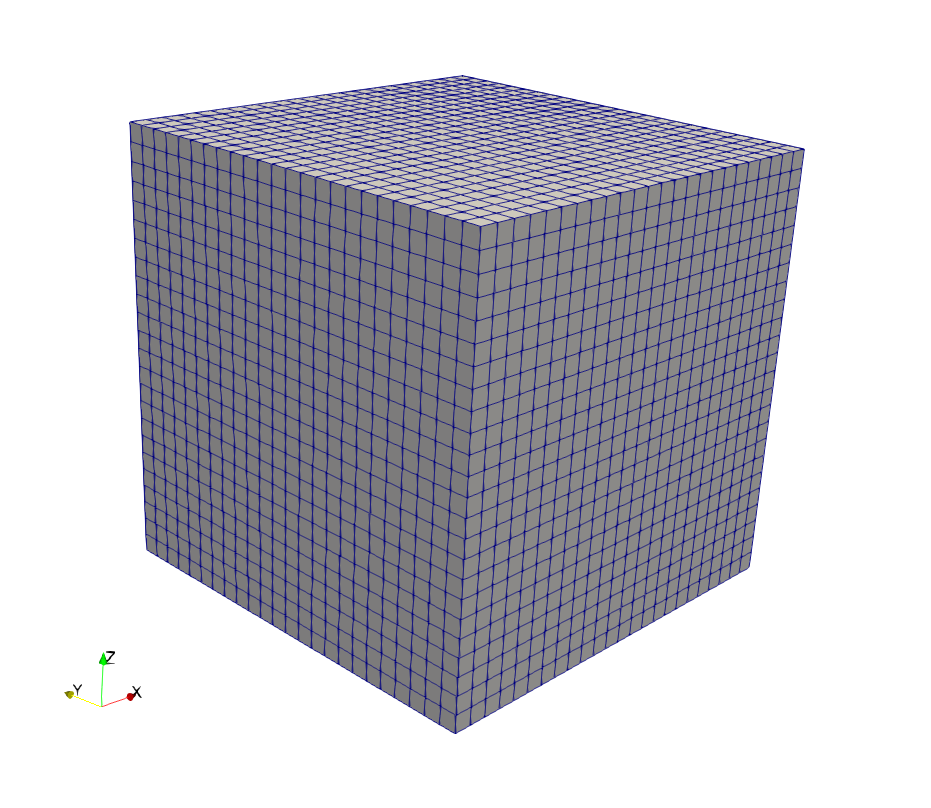
\includegraphics[width=5cm]{python_codes/fieldstone_stokes_sphere_3D/grid}
%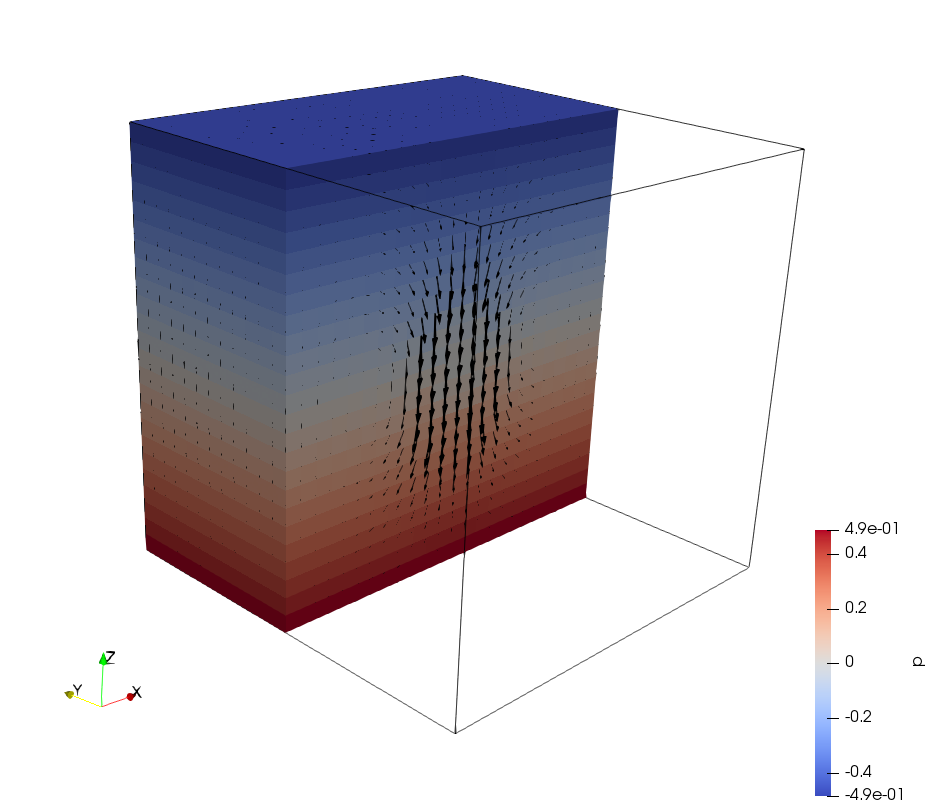
\includegraphics[width=5cm]{python_codes/fieldstone_stokes_sphere_3D/vel}
%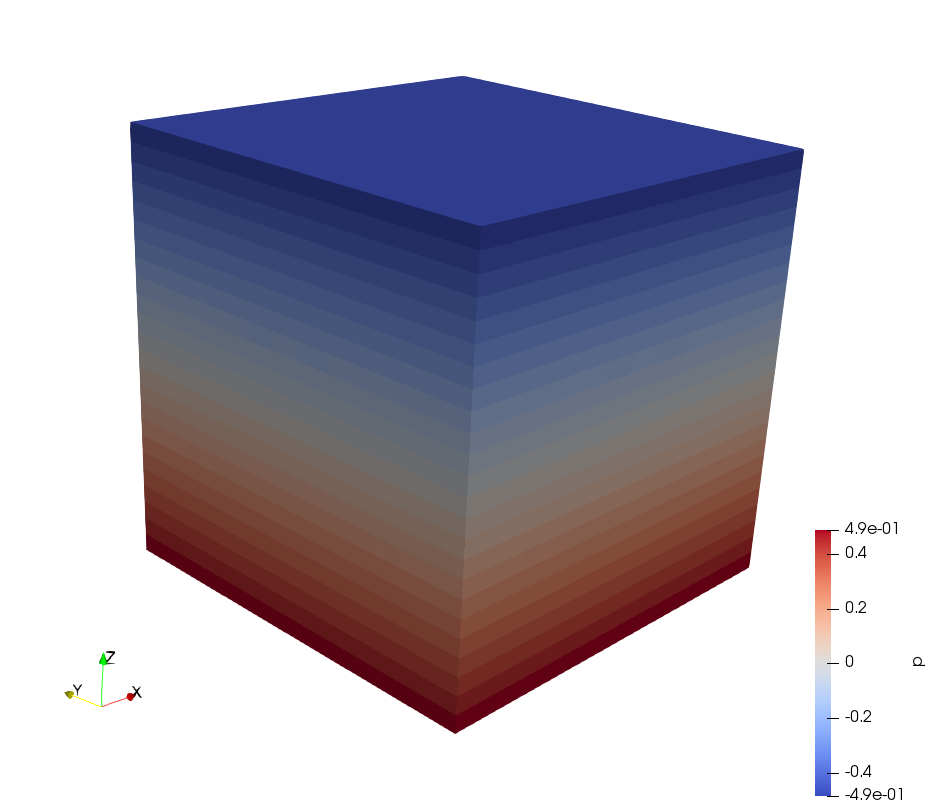
\includegraphics[width=5cm]{python_codes/fieldstone_stokes_sphere_3D/press}\\
%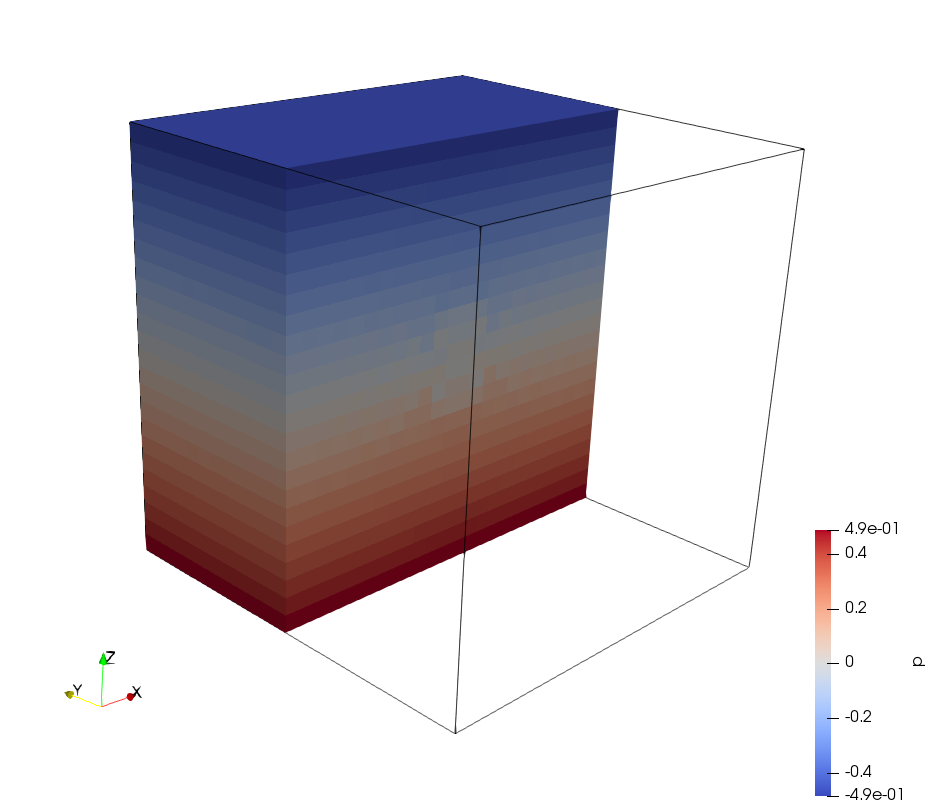
\includegraphics[width=5cm]{python_codes/fieldstone_stokes_sphere_3D/press2}
%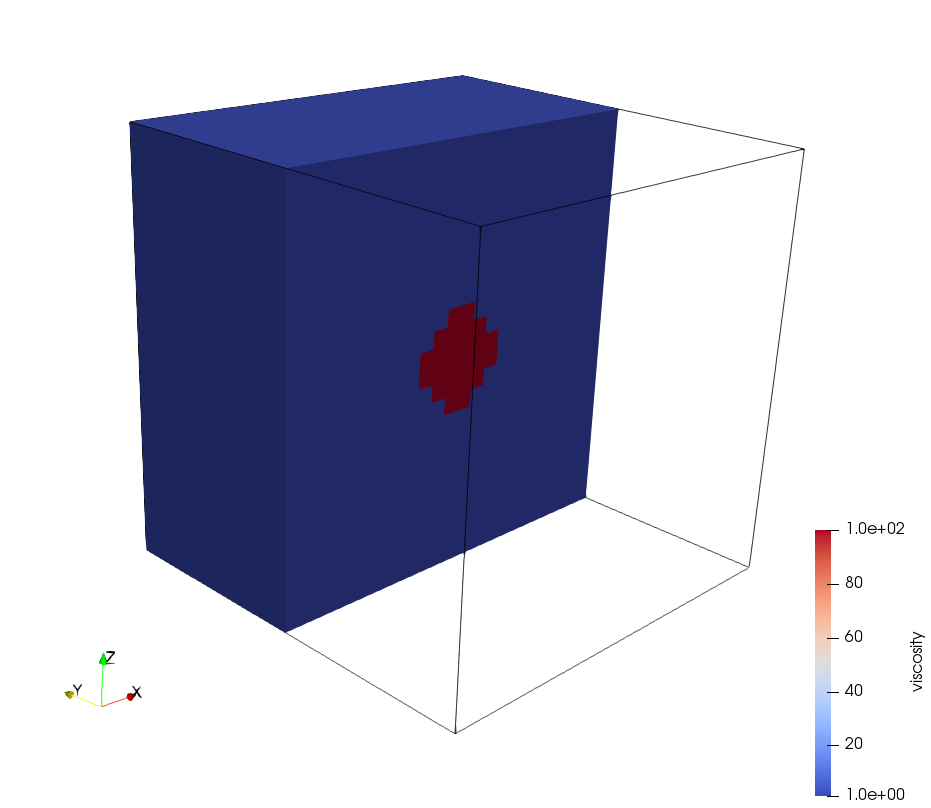
\includegraphics[width=5cm]{python_codes/fieldstone_stokes_sphere_3D/visc}
%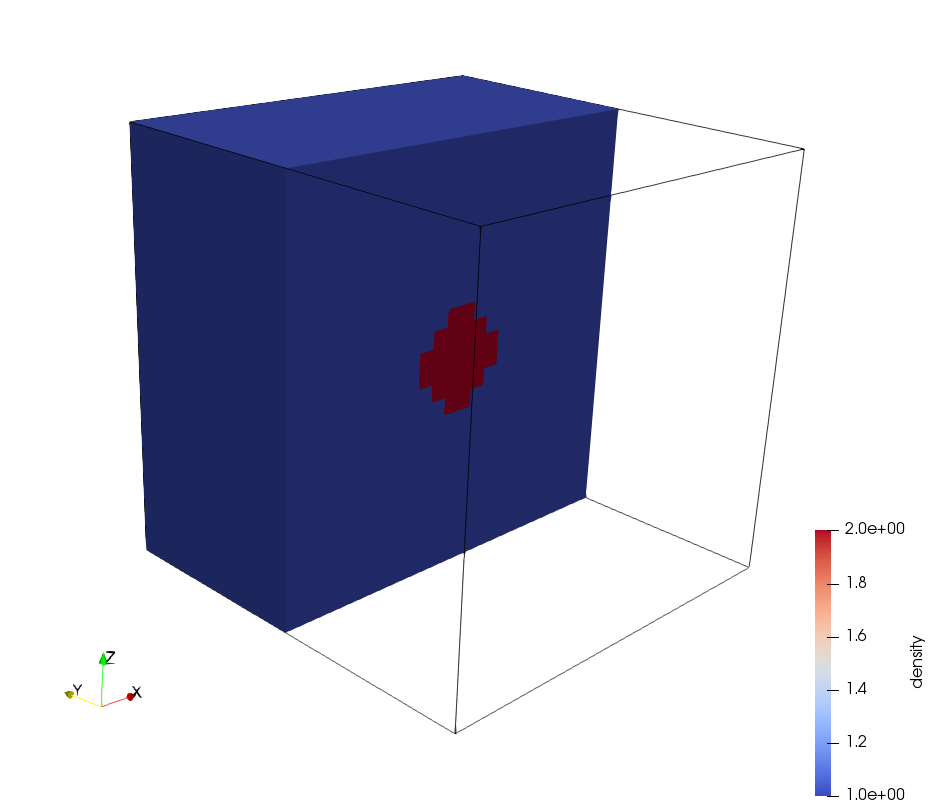
\includegraphics[width=5cm]{python_codes/fieldstone_stokes_sphere_3D/dens}\\
%{\small resolution is 24x24x24}
%\end{center}

